\section{本章の概要}
コンセプトマップ\cite{concept}とは,ある領域における概念をノードとして,関連性のあるノード同士を線,すなわちリンクで繋げたグラフ表現の内の一つである.
リンクには,ノードとノード間の関係性を表すリンクキーワードが設定されることもある.
コンセプトマップを用いることで,概念間の関係は視覚的に整理される.
視覚的に整理されるため,階層構造の理解に有効であるとされている.

\section{コンセプトマップについて}
コンセプトマップは,様々な分野で利用されているが,主に理科教育においてよく用いられている\cite{yama}\cite{saito}.
例えば以下の図は植物におけるコンセプトマップを作成した際の一例である.

\begin{figure}[htbp]
\begin{center}
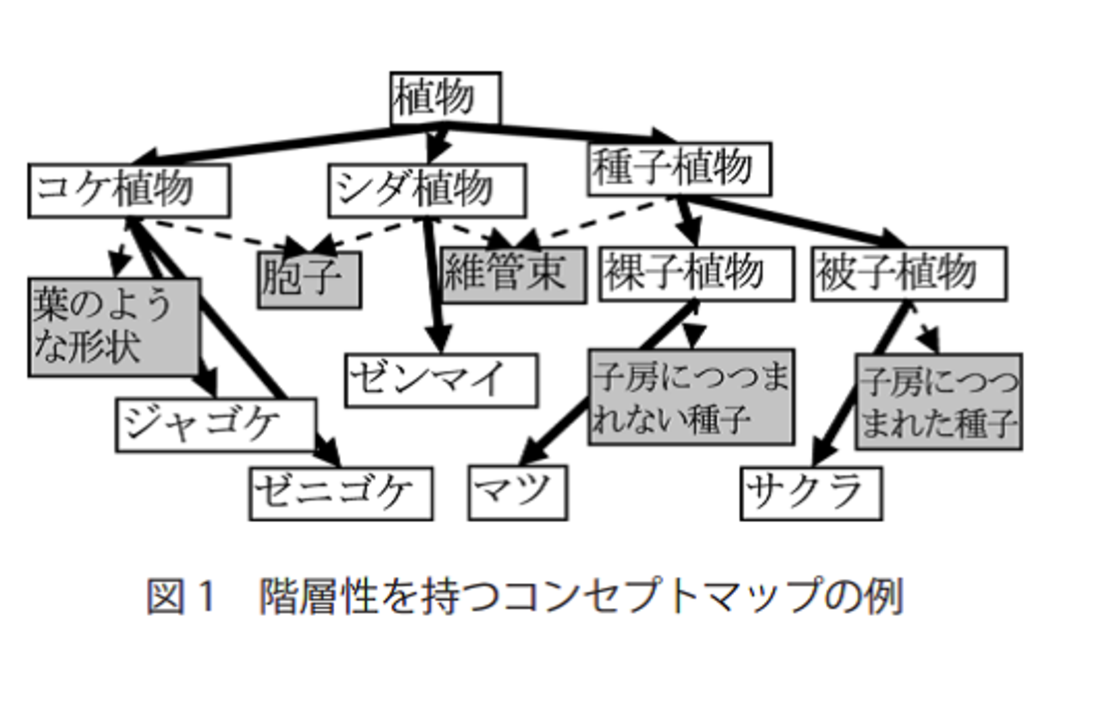
\includegraphics[width=8cm]{img/example_concept.eps}
\end{center}
\caption{コンセプトマップの例(出典: 誤りの可視化による階層構造の理解を指向したコンセプトマップ構築学習の支援環境 p.43 \cite{toumoto})}
\label{fig:example_concept}
\end{figure}